\documentclass[tikz, border=10pt]{standalone}
\usepackage{tikz}
\usetikzlibrary{calc}

\begin{document}
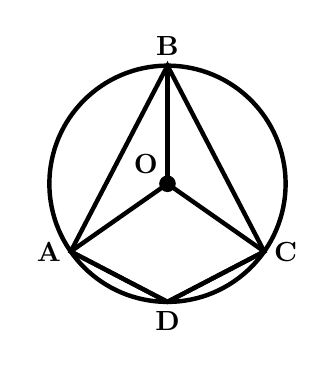
\begin{tikzpicture}

% Define radius
\def\r{1.5}

% Define center O
\coordinate (O) at (0, 0);

% Define points on the circle
\coordinate (B) at (90:\r);      % Top
\coordinate (A) at (215:\r);     % Bottom left
\coordinate (C) at (325:\r);     % Bottom right
\coordinate (D) at (270:\r);     % Bottom center

% Draw the circle
\draw[ultra thick] (O) circle (\r);

% Draw triangle ABC
\draw[ultra thick] (A) -- (B) -- (C) -- (D) -- cycle;

% Draw line AD
\draw[ultra thick] (A) -- (D);
\draw[ultra thick] (A) -- (O);
\draw[ultra thick] (C) -- (O);

% Draw line CD
\draw[ultra thick] (C) -- (D);

% Draw line OB (radius to top)
\draw[ultra thick] (O) -- (B);

% Draw center point O
\fill (O) circle (3pt);

% Labels
\node[above] at (B) {\textbf{B}};
\node[left] at (A) {\textbf{A}};
\node[right] at (C) {\textbf{C}};
\node[below] at (D) {\textbf{D}};
\node[above left] at (O) {\textbf{O}};

\end{tikzpicture}
\end{document}